\begin{apendicesenv}

\partapendices

\chapter{Gramática da linguagem FRED}
\label{sec:fredgrammar}

\begin{lstlisting}[caption=Gramática em notação LARK para linguagem FRED,label={lst:fredgrammar}]
document : stream
            | value

stream : "---" (value  "---")*

value : tagged
        | atom

tagged : name [attrs] atom
        | "(" name attr* ")" 

attrs : "(" attr* ")"

attr : name "=" atom

atom : object
        | array
        | date_time
        | symbol
        | number
        | string
        | bool
        | "null"

object : "{" pair* "}"

pair : name ":" value

array : "[" value* "]"

bool : "true" | "false"

symbol : "$" name

number : NUMBER_LITERAL 
        | HEX_LITERAL
        | OCT_LITERAL
        | BIN_LITERAL 

date_time : date
            | TIME_FORMAT

date : DATE_FORMAT [ ("_" | "T") TIME_FORMAT [ TIME_OFFSET ] ]

string : STRING_LITERAL
        | blob

blob : "#" BLOB_LITERAL

name : VARIABLE
        | QUOTED_VARIABLE

VARIABLE : /[^#\"`$:;{}\[\]=\(\)\t\r\n ,0-9]{1}[^#\"`$:;{}\[\]=\(\)\t\r\n ,]*/

QUOTED_VARIABLE : /`(?:[^\\`]|\\(?:[bfnrtv`\\/]|x[0-9a-fA-F]{2}|u[0-9a-fA-F]{4}|U[0-9a-fA-F]{8}))*`/

STRING_LITERAL : /"(?:[^\\"]|\\(?:[bfnrtv"\\/]|x[0-9a-fA-F]{2}|u[0-9a-fA-F]{4}|U[0-9a-fA-F]{8}))*"/

BLOB_LITERAL : /"(?:[^\\"\u\U]|\\(?:[bfnrtv"\\/]|x[0-9a-fA-F]{2}))*"/

NUMBER_LITERAL : /-?(0|[1-9]\d*)(\.\d+)?([eE][+-]?\d+)?/

HEX_LITERAL : /0x[0-9a-fA-F]{1}([0-9a-fA-F]{1}|_[0-9a-fA-F]{1})*/

OCT_LITERAL : /0o[0-8]{1}([0-8]{1}|_[0-8]{1})*/

BIN_LITERAL : /0b[01]{1}([01]{1}|_[01]{1})*/

DATE_FORMAT : /\d{4}-\d{2}-\d{2}/

TIME_FORMAT : /\d{2}:\d{2}:\d{2}(\.\d+)?/

TIME_OFFSET : /Z|[+-]\d{2}:\d{2}/

WHITESPACE : /[ \t\n\r,]+/

COMMENT : /;.*/
\end{lstlisting}

\chapter{Diagrama da Gramática da linguagem FRED}
\label{sec:fredtrain}

\begin{figure}[H]
	\centering
	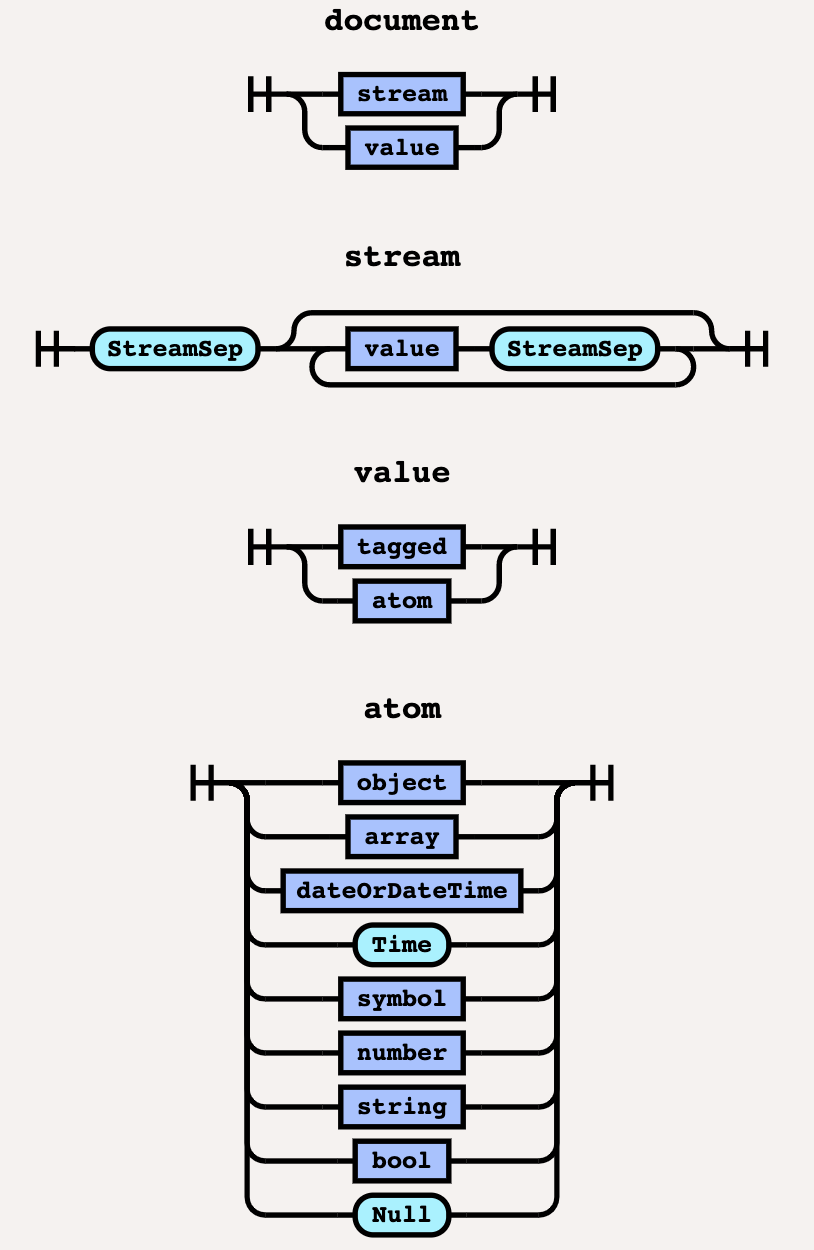
\includegraphics[keepaspectratio=true,scale=0.7]{figuras/syntaxdiagram1.png}
	\caption{Diagrama da Sintaxe do formato FRED (document até atom).}
\end{figure}

\begin{figure}[]
	\centering
	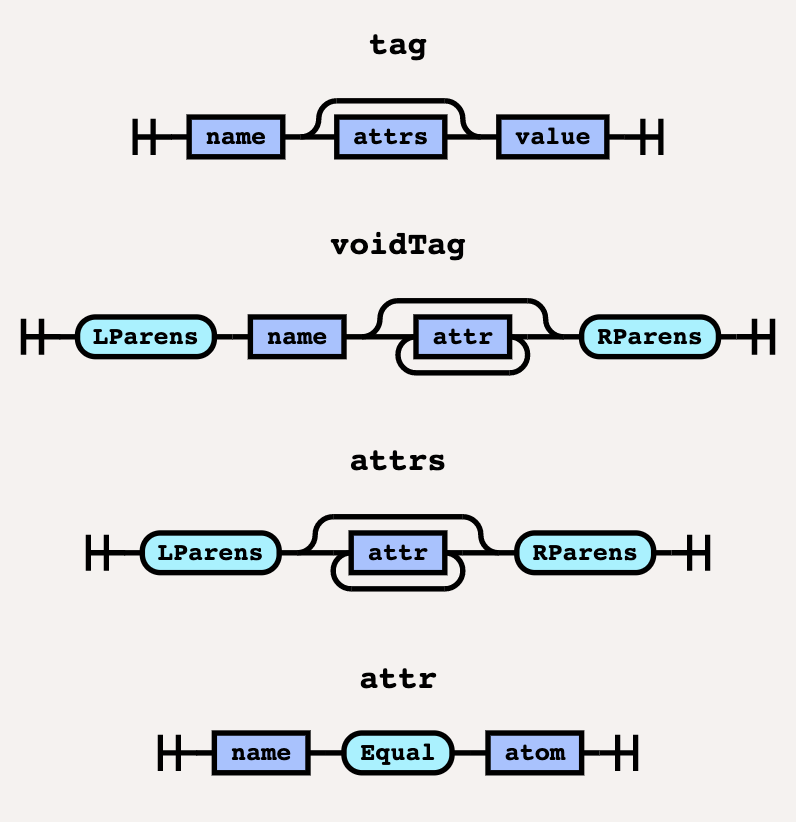
\includegraphics[keepaspectratio=true,scale=1]{figuras/syntaxdiagram2.png}
	\caption{Diagrama da Sintaxe do formato FRED (tag até attr).}
\end{figure}

\begin{figure}[]
	\centering
	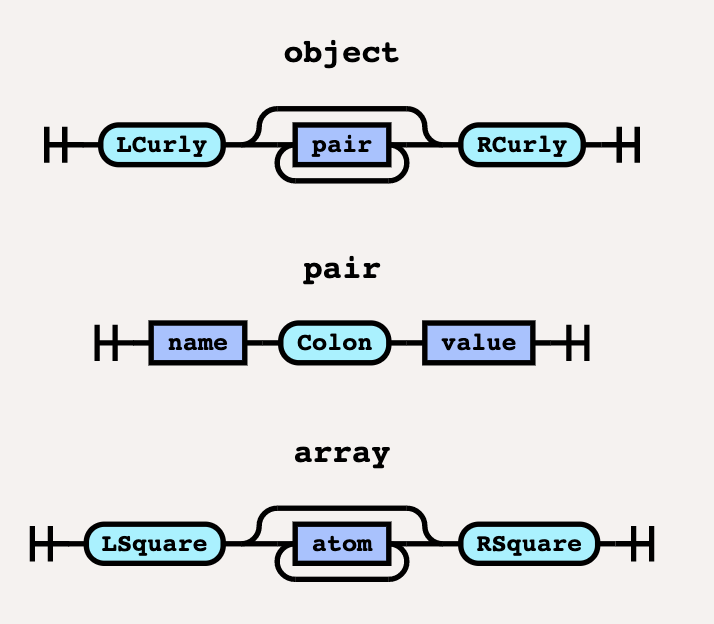
\includegraphics[keepaspectratio=true,scale=1]{figuras/syntaxdiagram3.png}
	\caption{Diagrama da Sintaxe do formato FRED (object até array).}
\end{figure}

\begin{figure}[]
	\centering
	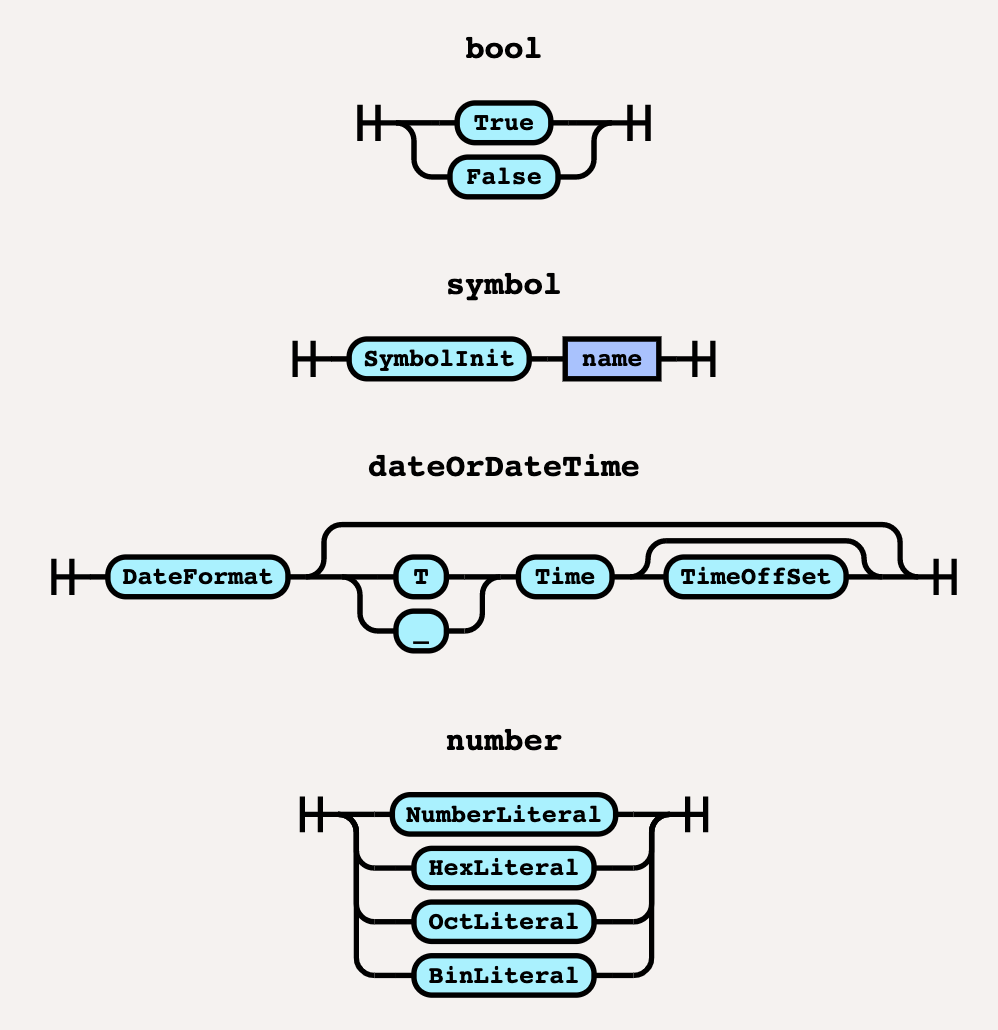
\includegraphics[keepaspectratio=true,scale=0.5]{figuras/syntaxdiagram4.png}
	\caption{Diagrama da Sintaxe do formato FRED (bool até number).}
\end{figure}

\begin{figure}[]
	\centering
	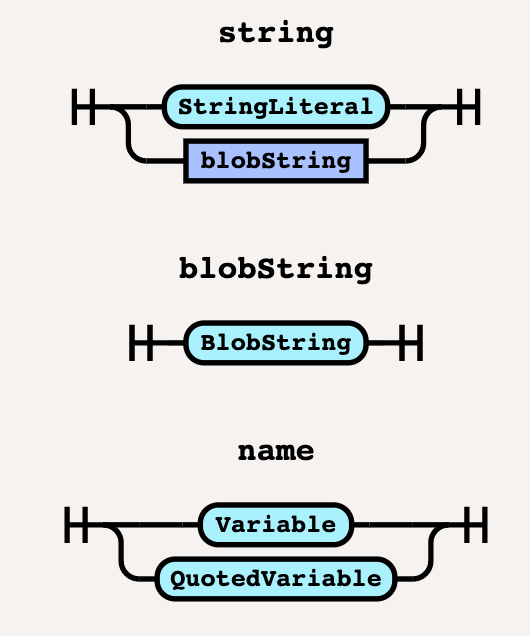
\includegraphics[keepaspectratio=true,scale=1]{figuras/syntaxdiagram5.png}
	\caption{Diagrama da Sintaxe do formato FRED (string até name).}
\end{figure}


\chapter{Documentos FRED, JSON e XML utilizados para comparação}
\label{sec:docsexamples}

\lstinputlisting[caption=Exemplo de documeto XML,label={lst:personxml}]{codigos/person.xml}

\lstinputlisting[caption=Exemplo de documeto JSON,label={lst:personjson}]{codigos/person.json}

\lstinputlisting[caption=Exemplo de documeto FRED,label={lst:personfred}]{codigos/person.fred}

\lstinputlisting[caption=Exemplo de documeto XML,label={lst:divxml}]{codigos/div.xml}

\lstinputlisting[caption=Exemplo de documeto JSON,label={lst:divjson}]{codigos/div.json}

\lstinputlisting[caption=Exemplo de documeto FRED,label={lst:divfred}]{codigos/div.fred}

\lstinputlisting[caption=Exemplo de documeto XML,label={lst:packagexml}]{codigos/package.xml}

\lstinputlisting[caption=Exemplo de documeto JSON,label={lst:packagejson}]{codigos/package.json}

\lstinputlisting[caption=Exemplo de documeto FRED,label={lst:packagefred}]{codigos/package.fred}

\end{apendicesenv}
